\documentclass{article}
\usepackage{graphicx} % Required for inserting images
\usepackage[left=4cm, right=4cm, top=4cm, bottom=4cm]{geometry}
\usepackage[T1]{fontenc}
\usepackage[polish]{babel}
\usepackage{amssymb}
\usepackage{url}
\usepackage{enumitem}
\usepackage{dirtree}
\usepackage[export]{adjustbox}
\usepackage{amsmath}
\usepackage{float}




\title{\Huge JIMP2 Projekt 2025 \\ {\huge Dokumentacja implementacyjna - Java}}
\author{Michał Ludwiczak \\ GR3}
\date{13 maja 2025}

\begin{document}

\maketitle

\tableofcontents



\section{Cel projektu}

    Celem projektu jest stworzenie aplikacji w języku Java, umożliwiającej podział grafu na określoną przez użytkownika liczbę części, z zachowaniem określonego lub domyślnego 10-procentowego marginesu różnicy liczby wierzchołków pomiędzy częściami. Domyślnie graf dzielony jest na dwie części. Celem podziału jest także minimalizacja liczby przeciętych krawędzi pomiędzy powstałymi częściami grafu. 
    Aplikacja będzie wyposażona w graficzny interfejs użytkownika wykonany w technologii Swing. Użytkownik będzie mógł wczytywać już podzielony graf z pliku tekstowego lub binarnego, wczytywać niepodzielone grafy, definiować liczbę części oraz margines podziału, a także zapisywać wynikowy graf wraz z danymi wejściowymi do pliku tekstowego lub binarnego. 
    Każda część grafu będzie prezentowana w interfejsie graficznym w odrębnym kolorze.
    
    \begin{figure}[H]
        \centering
        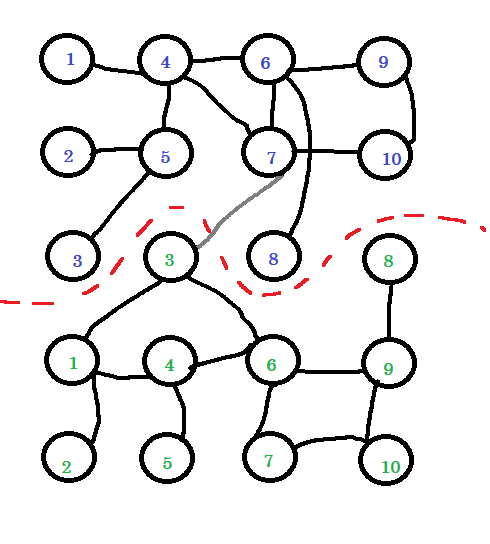
\includegraphics[width=0.75\linewidth]{img/graph.png}
        \caption{Przykładowy graf podzielony na 2 równe części}
        \label{fig:graph}
    \end{figure}



\section{Problem}

    Podział grafu na części w taki sposób, aby liczba przeciętych krawędzi była jak najmniejsza, nie jest problemem łatwym. Znalezienie optymalnego rozwiązania dla dużych grafów jest praktycznie niewykonalne w rozsądnym czasie, ponieważ liczba możliwych podziałów rośnie wykładniczo wraz z liczbą wierzchołków.
    W przypadku podziału grafu na dwie części istnieje \( 2^{n-1} - 1 \) możliwych sposobów podziału, gdzie \( n \) oznacza liczbę wierzchołków. Z tego powodu zamiast sprawdzania wszystkich możliwych podziałów stosuje się algorytmy przybliżone, heurystyki lub algorytmy zachłanne, które pozwalają na szybkie znalezienie dobrego, choć niekoniecznie optymalnego rozwiązania.

\section{Algorytm}

W programie zdecydowałem się użyć metody spektralnej dzielenia grafu, która wykorzystuje własności spektralne macierzy Laplace'a grafu. Na podstawie spektrum grafu, które opisuje jego strukturę graf możemy podzielić w efektywny i satysfakcjonujący sposób, minimalizując liczbę przeciętych krawędzi.


    \subsection{Macierz Laplace'a}
    
    W podejściu spektralnym do podziału grafu kluczową rolę odgrywa macierz Laplace'a \cite{laplacian_matrix}.
    Wzór na Laplacian klasyczny definiuje się jako:
    \[
    \mathbf{L} = \mathbf{D} - \mathbf{A}
    \]
    gdzie:
    \begin{itemize}
      \item \( L \) to \textbf{macierz Laplace'a} grafu,
      \item \( D \) to \textbf{macierz stopni} to macierz diagonalna, w której elementy na diagonali \( d_{ii} \) odpowiadają stopniowi wierzchołka \( i \), czyli liczbie krawędzi, które są z nim bezpośrednio połączone. W przypadku pętli, każda taka krawędź zwiększa stopień wierzchołka o 2, ponieważ jest traktowana jako dwie krawędzie incydentne z tym samym wierzchołkiem
      \item \( A \) to \textbf{macierz sąsiedztwa} grafu, gdzie elementy \( a_{ij} \) są równe 1, jeśli istnieje krawędź między wierzchołkami \( i \) i \( j \), oraz 0 w przeciwnym przypadku.
    \end{itemize}
    


    \subsection{Obliczenie par własnych}

    Następnym krokiem jest obliczenie \(k = p - 1\) (gdzie p to liczba części, na które graf ma być podzielony) najmniejszych wektorów własnych, nie wliczając pierwszego zerowego. Dla bisekcji będzie to tylko jeden wektor, drugi najmniejszy - wektor Fiedlera. Wektory własne macierzy Laplace'a grafu przechowują informacje o połączeniach pomiędzy wierzchołkami. Do obliczenia tych par własnych można posłużyć się biblioteką Smile/ARPACK. Jest oparta na metodzie Implicitly Restarted Arnoldi Method (IRAM) i zaprojektowana specjalnie do obliczania kilku wartości i wektorów własnych bardzo dużych, rzadkich macierzy CSR. Jednak dla macierzy Laplace'a grafu będzie wykorzystywać Implicitly Restarted Lanczos Method (IRLM) - IRAM dla symetrycznych macierzy, który stosuje metodę Lanczosa zamiast pełnej procedury Arnoldiego, budując tridiagonalną macierz $T_k$ oraz ortonormalną bazę wektorów własnych. Smile/ARPACK wymaga jedynie iloczynu macierz–wektor, co oznacza, że pamięć zajmowana jest proporcjonalnie do liczby niezerowych elementów, dzięki czemu świetnie sprawdza się przy analizie dużych grafów.



    \subsection{Podział}

    \subsubsection{Podział według wektora Fiedlera}
    Podział grafu według wektora Fiedlera polega na wykorzystaniu drugiego co do wielkości (drugiego najmniejszego) wektora własnego macierzy Laplasjanu grafu, nazywanego wektorem Fiedlera. Ten wektor koduje informację o strukturze spójności grafu – wierzchołki o podobnych wartościach współrzędnych wektora leżą blisko siebie w grafie.

    \subsubsection{Klasteryzacja}
    Natomiast po Po otrzymaniu macierzy zawierającej \(k\) wektorów własnych, każdy wierzchołek grafu jest reprezentowany jako punkt w \(k\)-wymiarowej przestrzeni. W celu podziału grafu na \(p\) części, można zastosować algorytm centroidów (k-means) \cite{k-means}.
    Centroidy są inicjalizowane na podstawie średniej wartości współrzędnych dla głównych osi. Następnie iteracyjnie przypisuje się wierzchołki do najbliższych centroidów, z uwzględnieniem limitu maksymalnej liczby elementów w jednym klastrze (wyznaczonego na podstawie dopuszczalnego marginesu). Po każdej iteracji aktualizowane są położenia centroidów, aż do równowagi.



    \subsection{Wynik}

    Po otrzymaniu poszczególnych części z wierzchołkami modyfikuje się macierz sąsiedztwa \(A\) usuwając krawędzie pomiędzy wierzchołkami przynależącymi do różnych grup. W ten sposób otrzymuje się nową macierz sąsiedztwa, która zawiera już podzielony graf. Macierz sąsiedztwa jest już gotowa do przetworzenia i wypisania na plik wyjściowy.
    


\section{Interfejs graficzny użytkownika}

    Aplikacja zostanie zaprojektowana z wykorzystaniem biblioteki Swing i oferuje graficzny interfejs użytkownika, który umożliwia interaktywną obsługę procesu podziału grafu. Interfejs składa się z następujących komponentów:

    \begin{itemize}
        \item \textbf{Ekran startowy} umożliwiający wybranie:
         \begin{itemize}
            \item \texttt{Wczytania grafu z pliku wejściowego, jego podzielenie po wybraniu liczby części i marginesu (w ekranie do \textbf{definicji podziału}), a następnie wyświetlenie}
            \item \texttt{Wczytanie podzielonego grafu z pliku wejściowego (wyjściowy z C) i jego wyświetlenie}
        \end{itemize}
        \begin{figure}[H]
            \centering
            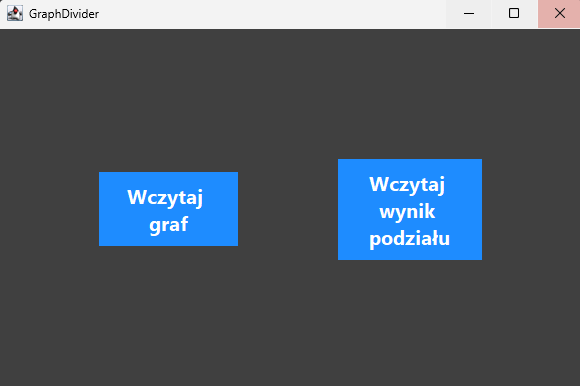
\includegraphics[width=0.9\linewidth]{img/start.png}
            \caption{Przykładowy ekran startowy}
            \label{fig:start}
        \end{figure}
        \item \textbf{Ekran do definicji podziału} z opcją wyboru liczby części i marginesu
        \item \textbf{Pasek menu lub przyciski} zawierające opcje:
        \begin{itemize}
            \item \texttt{Wczytaj z pliku tekstowego}
            \item \texttt{Wczytaj z pliku binarnego}
            \item \texttt{Zapisz wynik jako plik tekstowy}
            \item \texttt{Zapisz wynik jako plik binarny}
        \end{itemize}
        \item \textbf{Komponent prezentujący wczytany lub podzielony graf} \\
        Wierzchołki i krawędzie będą rysowane z wykorzystaniem metod graficznych Swing, a poszczególne części grafu po podziale są oznaczane różnymi kolorami.
        \item \textbf{Panel narzędziowy} zawierający:
        \begin{itemize}
            \item Pole do wprowadzenia liczby części, na które ma zostać podzielony graf (domyślnie 2).
            \item Pole do określenia dopuszczalnego marginesu procentowego różnicy w liczbie wierzchołków między częściami (domyślnie 10\%).
            \item Przycisk \texttt{Podziel graf}, który inicjuje proces podziału grafu zgodnie z podanymi parametrami.
        \end{itemize}
    \end{itemize}
    
    Interfejs zostanie zaprojektowany z myślą o intuicyjnej obsłudze, umożliwiając użytkownikowi łatwe wczytywanie grafów, definiowanie parametrów podziału oraz wizualizację wyników.
    
    \begin{figure}[H]
        \centering
        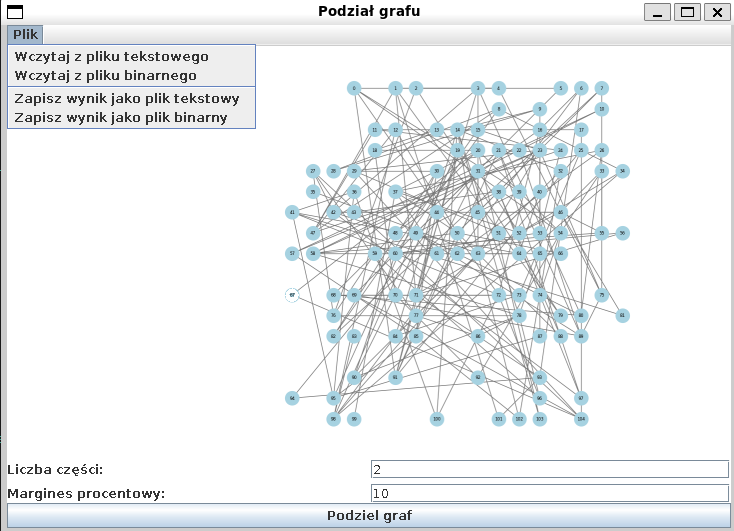
\includegraphics[width=0.9\linewidth]{img/interfejs.png}
        \caption{Przykładowy interfejs przed podziałem}
        \label{fig:interfejs}
    \end{figure}



\section{Struktura programu}

    W projekcie będę korzystał z Gradle jako głównego systemu budowania, co pozwoli na łatwe zarządzanie zależnościami i automatyzację procesu kompilacji. Wybranym IDE jest IntelliJ IDEA.
    
    \begin{itemize}
        \item \texttt{docs/} — katalog z dokumentacją
        \item \texttt{build.gradle} — główny plik konfiguracyjny Gradle
        \item \texttt{settings.gradle} — plik ustawień projektu
        \item \texttt{gradlew}, \texttt{gradlew.bat}, \texttt{gradle/wrapper/}
        \item \texttt{build/} — katalog generowany przez Gradle z artefaktami kompilacji
        \item \texttt{src/main/java/graphdivider/} — katalog dla właściwego programu w Java
          \begin{itemize}
              \item \texttt{gui/} - cały interfejs graficzny z wykorzystaniem biblioteki Swing
                    \begin{itemize}
                        \item \texttt{navigation/} - nawigacja odpowiedzialna za poszczególne ekrany
                            \begin{itemize}
                                 \item \texttt{Navigator.java}
                                 \item \texttt{AppNavigator.java}
                                 \begin{figure}[H]
                                        \centering
                                        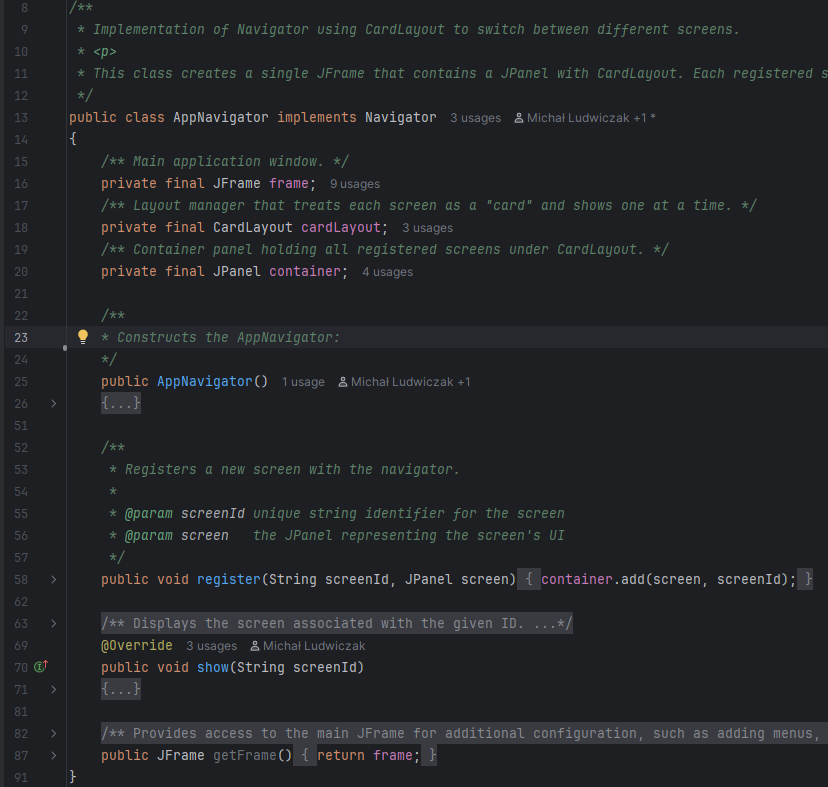
\includegraphics[width=0.9\linewidth]{img/appnavigator.png}
                                        \caption{AppNavigator.java}
                                        \label{fig:appnavigator}
                                 \end{figure}
                            \end{itemize}
                        \item \texttt{screen/} - poszczególne ekrany z zastosowaniem komponentów
                            \begin{itemize}
                                 \item \texttt{StartScreen.java} - ekran startowy
                                 \begin{figure}[H]
                                        \centering
                                        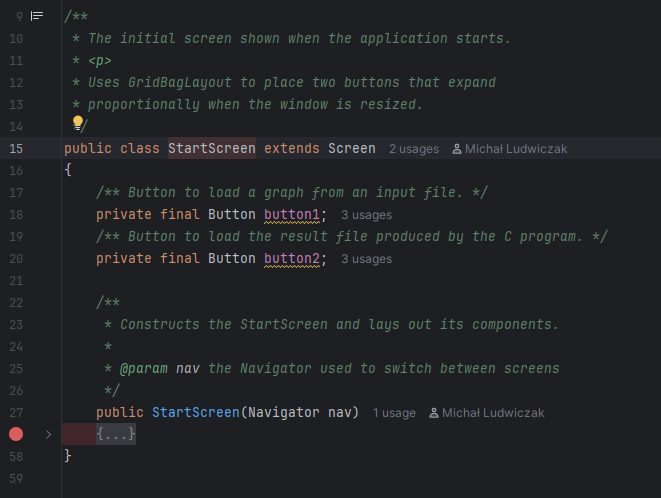
\includegraphics[width=0.9\linewidth]{img/startscreen.png}
                                        \caption{StartScreen.java}
                                        \label{fig:startscreen}
                                 \end{figure}
                                 \item \texttt{DivideScreen.java} - ekran podziału grafu
                                 \item \texttt{GraphScreen.java} - ekran wyświetlenia grafu
                            \end{itemize}
                        \item \texttt{widget/} - poszczególne komponenty Swing z zastosowaniem styli dla programu, w tym wizualizacja grafu
                            \begin{itemize}
                                 \item \texttt{Screen.java}
                                 \begin{figure}[H]
                                        \centering
                                        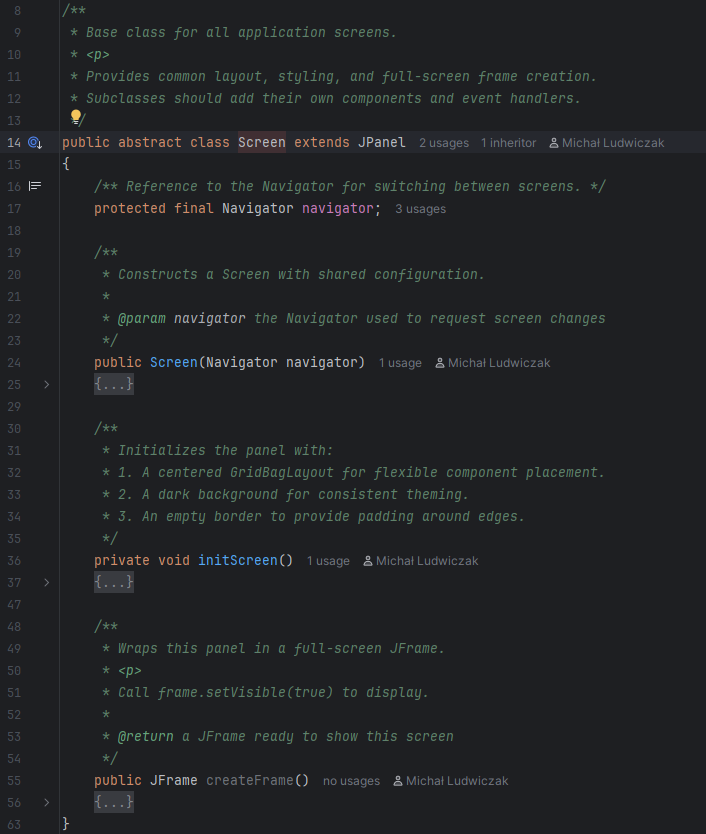
\includegraphics[width=0.9\linewidth]{img/screen.png}
                                        \caption{Screen.java}
                                        \label{fig:screen}
                                 \end{figure}
                                 \item \texttt{Button.java}
                                 \begin{figure}[H]
                                        \centering
                                        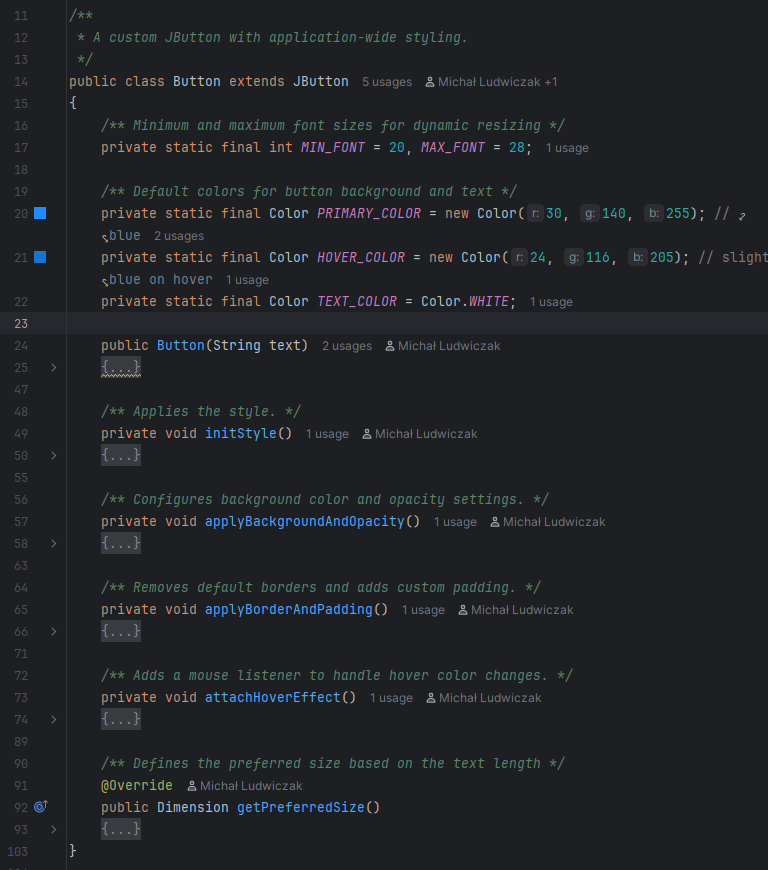
\includegraphics[width=0.9\linewidth]{img/button.png}
                                        \caption{Button.java}
                                        \label{fig:button}
                                 \end{figure}
                                 \item \texttt{Label.java}
                                 \item \texttt{Vertex.java}
                                 \item \texttt{Edges.java}
                                 \item \texttt{Graph.java}
                            \end{itemize}
                    \end{itemize}
              \item \texttt{algorithm/} - implementacja logiki algorytmu spektralnego
                    \begin{itemize}
                        \item \texttt{CSRmatrix.java} - reprezentacja grafu w postaci macierzy Laplace'a w formacie CSR, format CSR
                        \item \texttt{algorithm/} - implementacja właściwego algorytmu spektralnego
                            \begin{itemize}
                                \item \texttt{Eigenpairs.java} - obliczanie par własnych macierzy Laplace'a grafu
                                \item \texttt{Clusterization.java} - klasteryzacja - podział grafu
                            \end{itemize}
                        \item \texttt{Output.java} - wypisanie do pliku wyjściowego
                    \end{itemize}
              \item \texttt{Main.java} - wywoływanie całego programu i poszczególnych modułów
          \end{itemize}
          \item \texttt{src/main/resources/} — katalog z zasobami
                \begin{itemize}
                    \item \texttt{input/} - pliki wejściowe
                    \item \texttt{input\_c/} - pliki wejściowe (wyjściowe z programu w C)
                    \item \texttt{icon.png} - ikonka programu
                \end{itemize}
    \end{itemize}

        



\section{Pliki wejściowe i wyjściowe dla trybu dzielenia}

    \subsection{Plik wejściowy (\texttt{.csrrg} / \texttt{.bin})}
    
    Wejście programu może przyjąć dwie formy:
    \begin{itemize}
        \item Plik \texttt{.csrrg} z dodatkowymi sekcjami po piątej linii, opisującymi kolejne podgrafy powstałe z podziału grafu.
        Format pliku składa się z pięciu sekcji zapisanych w kolejnych liniach:
        \begin{enumerate}
            \item Maksymalna liczba wierzchołków w dowolnym wierszu macierzy sąsiedztwa.
            \item Lista sąsiadów wszystkich wierzchołków zapisana sekwencyjnie.
            \item Wskaźniki (indeksy) na początki list sąsiedztwa dla poszczególnych wierzchołków.
            \item Lista grup wierzchołków połączonych krawędziami (reprezentacja krawędzi).
            \item Wskaźniki na początki grup węzłów z poprzedniej listy.
        \end{enumerate}
        \item Plik binarny \texttt{.bin} — binarna forma pliku \texttt{.csrrg}, mniej czytelna dla człowieka, ale szybsza w odczycie przez program.
    \end{itemize}
    
    \subsection{Plik wyjściowy (\texttt{.csrrg2} / \texttt{.bin})}

    Po przetworzeniu danych program generuje plik wyjściowy w jednym z dwóch formatów:
    \begin{itemize}
        \item \texttt{.csrrg2} — tekstowa forma pliku wyjściowego, wzorowana na formacie wejściowym .csrrg, ale zawierająca dodatkową linię nagłówkową z wynikiem działania programu.
        \item \texttt{.bin} — binarna wersja pliku tekstowego \texttt{.csrrg2}.
    \end{itemize}
    
    W pierwszej linii pliku wyjściowego zapisywany jest rezultat działania programu w formacie:
    \begin{center}
    \texttt{<wynik (S - sukces, F - porażka)> <liczba\_części> <liczba\_przecięć> <zachowany\_margines>}
    \end{center}
    Przykład:
    \begin{center}
    \texttt{S 3 2 5}
    \end{center}
    


\section{Pliki wejściowe dla trybu wyświetlenia podzielonego grafu}
    (pliki wyjściowe programu w C)

    \subsection{Plik wejściowy w formacie \texttt{.csrrg}}
    Plik przyjmuje postać taką jak plik wejściowy w formacie .csrrg z tym, że linijki po 5 linijce zawierają wierzchołki należące do danych kolejnych podgrup.
    \begin{figure}[H]
        \centering
        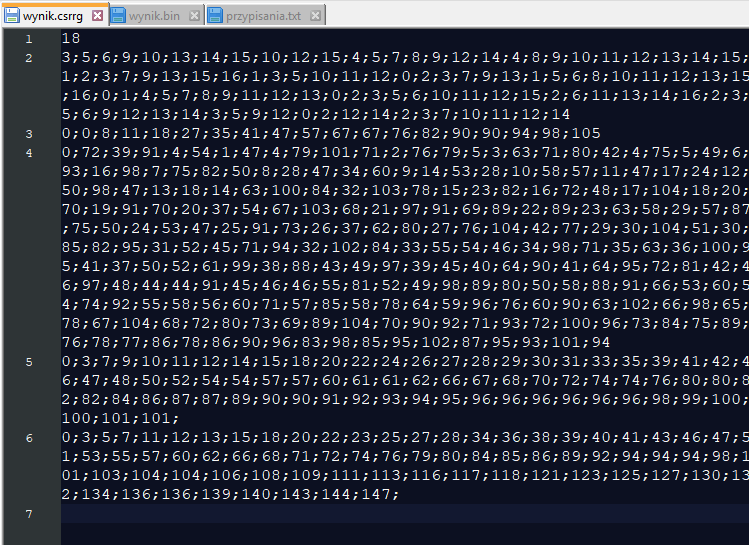
\includegraphics[width=0.9\linewidth]{img/plik_c.png}
        \caption{Przykładowy plik wejściowy dla trybu wyświetlenia}
        \label{fig:plik_c}
    \end{figure}

    \subsection{Plik wejściowy w formacie binarnym (\texttt{.bin})}
    Zapis taki sam jak w formacie .csrrg.

    



\section{Przykłady użycia}

    \subsection{Wczytywanie grafu z pliku tekstowego}
    
    Aby wczytać graf z pliku tekstowego \texttt{graf.csrrg}, wybierz opcję \texttt{Wczytaj z pliku tekstowego} z paska menu. Program odczyta dane grafu, a następnie wyświetli je w głównym obszarze aplikacji.

    \subsection{Wczytywanie grafu z pliku binarnego}
    
    Aby wczytać graf z pliku binarnego \texttt{graf.bin}, wybierz opcję \texttt{Wczytaj z pliku binarnego} z paska menu. Program odczyta dane grafu w formacie binarnym i wyświetli je w głównym obszarze aplikacji.
    
    \subsection{Podział grafu na x części z marginesem y}
    
    Po załadowaniu grafu, w panelu narzędziowym ustaw liczbę części na \texttt{x} oraz margines na \texttt{y\%}. Następnie kliknij przycisk \texttt{Podziel graf}, aby rozpocząć proces podziału. Program spróbuje podzielić graf na x części, minimalizując liczbę przeciętych krawędzi, z zachowaniem określonego marginesu różnicy liczby wierzchołków.
    
    \subsection{Zapisanie wyniku do pliku wyjściowego}
    
    Po zakończeniu podziału, aby zapisać wynik do pliku tekstowego, wybierz opcję \texttt{Zapisz wynik jako plik tekstowy} z paska menu. Program zapisze dane grafu w formacie \texttt{.csrrg2}, zawierającym dodatkową linię nagłówkową z wynikiem działania programu.
    
    \subsection{Zapisanie wyniku do pliku binarnego}
    
    Po zakończeniu podziału, aby zapisać wynik do pliku binarnego, wybierz opcję \texttt{Zapisz wynik jako plik binarny} z paska menu. Program zapisze dane grafu w formacie \texttt{.bin}, co pozwoli na szybszy odczyt danych w przyszłości.



\section{Wymagania niefunkcjonalne}

    Poniżej przedstawiono kluczowe wymagania niefunkcjonalne dla aplikacji:
    
    \begin{itemize}
        \item \textbf{Wydajność:} Czas podziału grafu powinien być jak najkrótszy dla danej wielkości grafu. Dla grafów zawierających do 1000 wierzchołków, czas przetwarzania nie powinien przekraczać minuty na standardowym sprzęcie klasy PC.
        \item \textbf{Użyteczność:} Interfejs użytkownika powinien być intuicyjny i zgodny z ogólnie przyjętymi standardami projektowania GUI.
        \item \textbf{Skalowalność:} Aplikacja powinna umożliwiać obsługę grafów o różnej wielkości, od małych do dużych.
        \item \textbf{Przenośność:} Aplikacja powinna działać poprawnie na różnych systemach operacyjnych wspierających środowisko Java.
        \item \textbf{Utrzymywalność:} Kod źródłowy aplikacji powinien być czytelny i dobrze udokumentowany, aby ułatwić przyszłe modyfikacje i rozwój.
    \end{itemize}


    

\begin{thebibliography}{9}

\bibitem{youtube_video}
Leonid Zhukov, \textit{Lecture 7. Graph partitioning algorithms.}, YouTube, 24 luty 2021, Dostępny na 11 maja 2025 w: \url{https://youtu.be/zZae_C2BU_4}

\bibitem{laplacian_matrix}
\textit{Laplacian matrix}, Wikipedia, Dostępne na 11 maja 2025 w: \url{https://en.wikipedia.org/wiki/Laplacian_matrix}

\bibitem{k-means}
\textit{Algorytm centroidów}, Wikipedia, Dostępne na 11 maja 2025 w:
\url{https://pl.wikipedia.org/wiki/Algorytm_centroid%C3%B3w}

\end{thebibliography}


\end{document}
